\documentclass[aps,prl,amsmath,amssymb,preprint,superscriptaddress]{revtex4}

\usepackage{graphicx}% Include figure files
\usepackage{dcolumn}% Align table columns on decimal point
\usepackage{bm}% bold math

% Alter some LaTeX defaults for better treatment of figures:
    % See p.105 of "TeX Unbound" for suggested values.
    % See pp. 199-200 of Lamport's "LaTeX" book for details.
    %   General parameters, for ALL pages:
    \renewcommand{\topfraction}{0.9}    % max fraction of floats at top
    \renewcommand{\bottomfraction}{0.8}    % max fraction of floats at bottom
    %   Parameters for TEXT pages (not float pages):
    \setcounter{topnumber}{2}
    \setcounter{bottomnumber}{2}
    \setcounter{totalnumber}{4}     % 2 may work better
    \setcounter{dbltopnumber}{2}    % for 2-column pages
    \renewcommand{\dbltopfraction}{0.9}    % fit big float above 2-col. text
    \renewcommand{\textfraction}{0.07}    % allow minimal text w. figs
    %   Parameters for FLOAT pages (not text pages):
    \renewcommand{\floatpagefraction}{0.7}    % require fuller float pages
    % N.B.: floatpagefraction MUST be less than topfraction !!
    \renewcommand{\dblfloatpagefraction}{0.7}    % require fuller float pages
    % remember to use [htp] or [htpb] for placement
    \setlength{\abovecaptionskip}{0pt}
    \setlength{\belowcaptionskip}{0pt}
    \setlength{\parskip}{0pt}
    \setlength{\textfloatsep}{1pt} 

\begin{document}
%\title{Reduction of turbulent fluctuations and crossphase through driven sheared flow on the Large Plasma Device}
\title{Observation of improved and degraded confinement with driven flow on the LAPD}
\author{D.A. Schaffner}
\affiliation{Department of Physics and Astronomy, University of California, Los Angeles.}
\author{T.A Carter}
\affiliation{Department of Physics and Astronomy, University of California, Los Angeles.}
\author{G.D. Rossi}
\affiliation{Department of Physics, University of Texas, Austin}
\author{D.S. Guice}
\affiliation{Department of Physics and Astronomy, University of California, Los Angeles.}
\author{J. Maggs}
\affiliation{Department of Physics and Astronomy, University of California, Los Angeles.}
\author{S. Vincena}
\affiliation{Department of Physics and Astronomy, University of California, Los Angeles.}
\author{B. Friedman}
\affiliation{Department of Physics and Astronomy, University of California, Los Angeles.}


\date{\today}

\begin{abstract}
Continuous control over azimuthal flow and shear in the edge of the Large Plasma Device (LAPD) has been acheived using a biasable limiter which has allowed a careful study of the effect of flow shear on pressure-gradient-driven turbulence and transport in LAPD. LAPD rotates spontaneously in the ion diamagnetic direction (IDD); positive limiter bias first reduces, then minimizes (producing a near-zero shear state), and finally reverses the flow into the electron diamagnetic direction (EDD). Degradation of particle confinement is observed in the minimum shearing state and reduction in turbulent particle flux is observed with increasing shearing in both flow directions. Near-complete suppression of turbulent particle flux is observed for shearing rates comparable to the turbulent autocorrelation rate measured in the minimum shear state.  Turbulent flux suppression is dominated by amplitude reduction in low-frequency ($>10$kHz) density fluctuations and a reduction in the radial correlation length. An increase in fluctuations for the highest shearing states is observed with the emergence of a coherent mode which does not lead to net particle transport. The variations of density fluctuation and radial correlation length are fit well with power-laws and compare favorably to simple models of shear suppression of transport.
\end{abstract}

\maketitle
%\section{Introduction}  No need for section titles in PRL, save space

%% Need to start with discussion of H-mode, role of flow.  Cite BDT, recent reviews of flow-shear interaction (Terry, Diamond, Tynan).  Move immediately to set up why this study is uni

While flow shear does provide a source of free energy for instability and turbulence~\cite{}, it can lead to stabilization of pressure-gradient-driven instabilities and a reduction of turbulent transport in magnetized plasmas~\cite{Burrell:1997, Terry:2000}.  The transport barrier in the high-confinement mode, or H-mode, of tokamak operation~\cite{wagner82} is attributed to the spontaneous development of a edge flow layer in which  strong shearing suppresses transport~\cite{burrell, terry, hahm?}.  The direct connection between the H-mode edge flow layer and improved confinement was first established in experiments on the Continuous Current Tokamak (CCT) in which transport barriers were generated by directly driving edge flow using torque due to radial currents driven by biased electrodes~\cite{taylor89,tynan92}.  Biasing has been used to produce improved confinement in a number of subsequent experiments including toroidal devices~\cite{Weynants:1992,Boedo:2000,Silva:2006,Craig:1997,Chapman:1998,Shats:2000} and linear magnetized plasmas~\cite{Sakai:1993,maggs07,carter09}.  
Turbulence can self-regulate through the generation of flows and flow
shear (zonal flows); this effect is often invoked to explain
saturation of drift turbulence and as a possible explanation for
spontaneous confinement transitions in fusion
devices~\cite{Terry:2000,Diamond:2005}.  Direct evidence for
turbulent-Reynolds-stress-driven flow has been reported in a
cylindrical magnetized plasma device~\cite{Holland:2006}. 


While ample evidence for transport reduction in the presence of
sheared flow exists~\cite{Burrell:1999, Tynan:2009} and significant
effort and progress has been made in developing a theoretical
understanding the interaction between sheared flow and turbulence,
there are still a number of open questions that can be answered by
experiment.  In particular, the exact mechanism behind turbulence
modification and transport suppression occur in the presence of shear
is still subject to debate: theories present a number of mechanisms
including radial decorrelation~\cite{Biglari:1990}, nonlinear reduction of
turbulent amplitude~\cite{Kim:2004}, and modification of turbulent
cross-phase~\cite{Ware:1996}.  Evidence for all of these mechanisms exists in
experimental data~\cite{Tynan:2009}, but a comprehensive experimental
dataset establishing in detail the parameter regimes where each
mechanism is important has not been acquired.  In part, this is due o
the fact that most datasets on flow-turbulence interaction come from
studies of spontaneously generated flow or in cases where precise
external control over flow and flow shear is not possible.  A number
of basic plasma experiments have utilized biasing techniques to drive
flow and flow shear to study flow driven
instabilities (e.g. \cite{Amatucci:1996,Jassby:1970}),
however experiments have not been successfully done in which precise external
control over flow and flow shear has been achieved in the presence of
drift-wave turbulence to systematically study the changes in
turbulence characteristics and transport.

In this letter, we report on the first experiments in which external
control of flow is used to document the response of turbulence and
transport to a continuous variation of flow shear, including a zero
shear state and a reversal of the flow direction.  
Shearing rates ($\omega_{s}= \partial V_{\theta}/\partial r$) from
zero to up to five times the turbulent autocorrelation rate measured
at zero flow shear ($\Delta \omega_{d}$) are achieved. Turbulent
particle flux is reduced with increasing shearing rate, regardless of the
direction of the flow or sign of the flow shear, with significant
reduction occuring for $\omega_s \sim \Delta \omega_d$.  The observed
reduction in particle flux is dominated by decreases in low-frequency
($f < 10$kHz) density fluctuation amplitude and a reduction of the
radial correlation length is also observed. For low frequency
fluctuations, the crossphase
between density and azimuthal electric field fluctuations remain near
zero for all shearing rates.  With higher shear ($\omega_s > \Delta
\omega_d$) we observe the emergence of a coherent mode localized spatially in the region
of strong flow. Fluctuations from this mode appear to increase density
fluctuations above 10kHz, but do not appear to contribute to particle
flux.   
%we show fits
%of density fluctuations and radial correlation length to a power-law
%decay for comparison to a simple theory \cite{biglari90}.

The Large Plasma Device \cite{gek91} (LAPD) is a 17m long, $\sim 60$cm
diameter cylindrical plasma produced by a barium-oxide coated nickel
cathode. In the experiments reported here, a plasma of density $\sim 5
\times 10^{12}$ cm$^{-3}$ and peak temperature of $\sim 8 eV$ is
produced in a uniform magnetic field of 1000G.  Measurements of 
electron density, electron temperature, and potential (both plasma
potential and floating potential) are made using Langmuir probes.  
Measurements of ion saturation current ($I_{\rm sat} \propto n_e \sqrt{T_e}$) and floating
potential ($V_f$) are taken with a 9-tip Langmuir probe (flush-mount
tantalum tips) probe while temperature and plasma potential is
determined using a swept Langmuir probe. Turbulent particle flux
$\Gamma = \left<\tilde{n}_e \tilde{E}_\theta\right>$ is
determined through correlating $I_{\rm sat}$ fluctuations from one tip
of this probe with
azimuthal electric field fluctuations ($E_\theta$) derived from
floating potential fluctuations on two azimuthally separated tips.
Azimuthal $E\times B$ flow is computed
using the swept-probe-derived plasma potential.  Flows derived using
this technique during these experiments compare very well to measurements using
Mach probes~\cite{maggs2007} and flows derived from time-delay
estimation (TDE) of the velocity of turbulent structures~\cite{}.
  
Biasing experiments have been previously conducted on LAPD in which edge profile steepening and a reduction in turbulent flux was observed~\cite{maggs07,carter09}. In these experiments, edge flow was driven through biasing the vacuum chamber wall with respect to the plasma source cathode.  Transport reduction occurred only for biases above a threshold value.  Below the threshold, azimuthal flow was localized near the biased wall and no flow or flow shear was driven in the region where drift wave turbulence exists.  Above the threshold, the flow was able to penetrate radially inward and strong flow and flow shear, with shearing rate far above the low-flow turbulent autocorrelation rate, was driven in the region of strong density gradient.   Recent experiments were successful in more continuous control of potential and cross-field flow in the shadow of a biased obstacle inserted into the LAPD core plasma~\cite{zhou12}.  Both confinement improvement and degradation (formation of strong density depletions) were observed with the density profile created by the obstacle in this case.  

Building on the success of biasing obstacles to control flow, an annular aluminum limiter was installed in LAPD. The provides a parallel boundary condition for the edge plasma and is biased relative to the cathode of the plasma source to control plasma potential and cross-field flow.  The limiter is
an iris-like design with four movable plates and is located ??? m from
the cathode.  In these experiments, the limiter plates were adjusted
to provide a provide a 52cm diameter aperture; downstream of the
limiter, plasma on field lines with radial location $r>26$cm sees the
limiter as a conducting end boundary condition and plasma on field
lines for $r<26$cm sees the anode/cathode of the source region as a
parallel boundary condition.  A capacitor back connected to a transistor switch supplies a bias voltage pulse to the limiter.  The
bias pulse lasted 5ms during the flattop of the $\sim 15$ms plasma
discharge. The limiter was biased from $\sim 10$V below the anode
potential to 50V above the anode voltage.  Typically plasma potential
in the core LAPD plasma (plasma on field lines that connect to the
source region) is very close to the anode voltage and the cathode sits
near ground (vacuum chamber wall).  The anode potential is above the
cathode potential by the discharge voltage, which was XXX during these experiments.

\begin{figure}[!htbp]
\centerline{
\includegraphics[width=8.5cm]{velocity_flowshear.pdf}}
\caption{\label{fig:velocity_flowshear} (a) Velocity profiles using plasma potential from swept measurements. (b) Nearly linear scaling of flow (black) and shearing (red) versus limiter bias. Note that the zero in mean absolute shear does not occur at zero average flow.}
\end{figure}

Spontaneous rotation of the LAPD is observed when the limiters are
unbiased (here the limiters are observed to float to a
potential $\sim 10$V below the anode).  In this state, an edge flow
(peaked just outside the limiter edge) is
observed in the ion diamagnetic direction (IDD), as shown in
Fig.~\ref{fig:velocity_flowshear}(a).  Biasing the limiter positively
with respect to the cathode tends to drive flow in the electron
diamagnetic direction (EDD).  As the limiter bias is increased, the
flow in the IDD is first reduced, then reaching near-zero flow
and flow-shear states, and is ultimately reversed with strong EDD flow.

Measurements of profiles of density ($I_{\rm sat}$) and particle flux
were made for each bias flow state. Values are averaged over a range
from 27 to 31cm, a region where average flow and flow shear scale
nearly linearly with limiter bias, as shown in
Fig.~\ref{fig:velocity_flowshear}(b).  

\begin{figure}[!htbp]
\centerline{
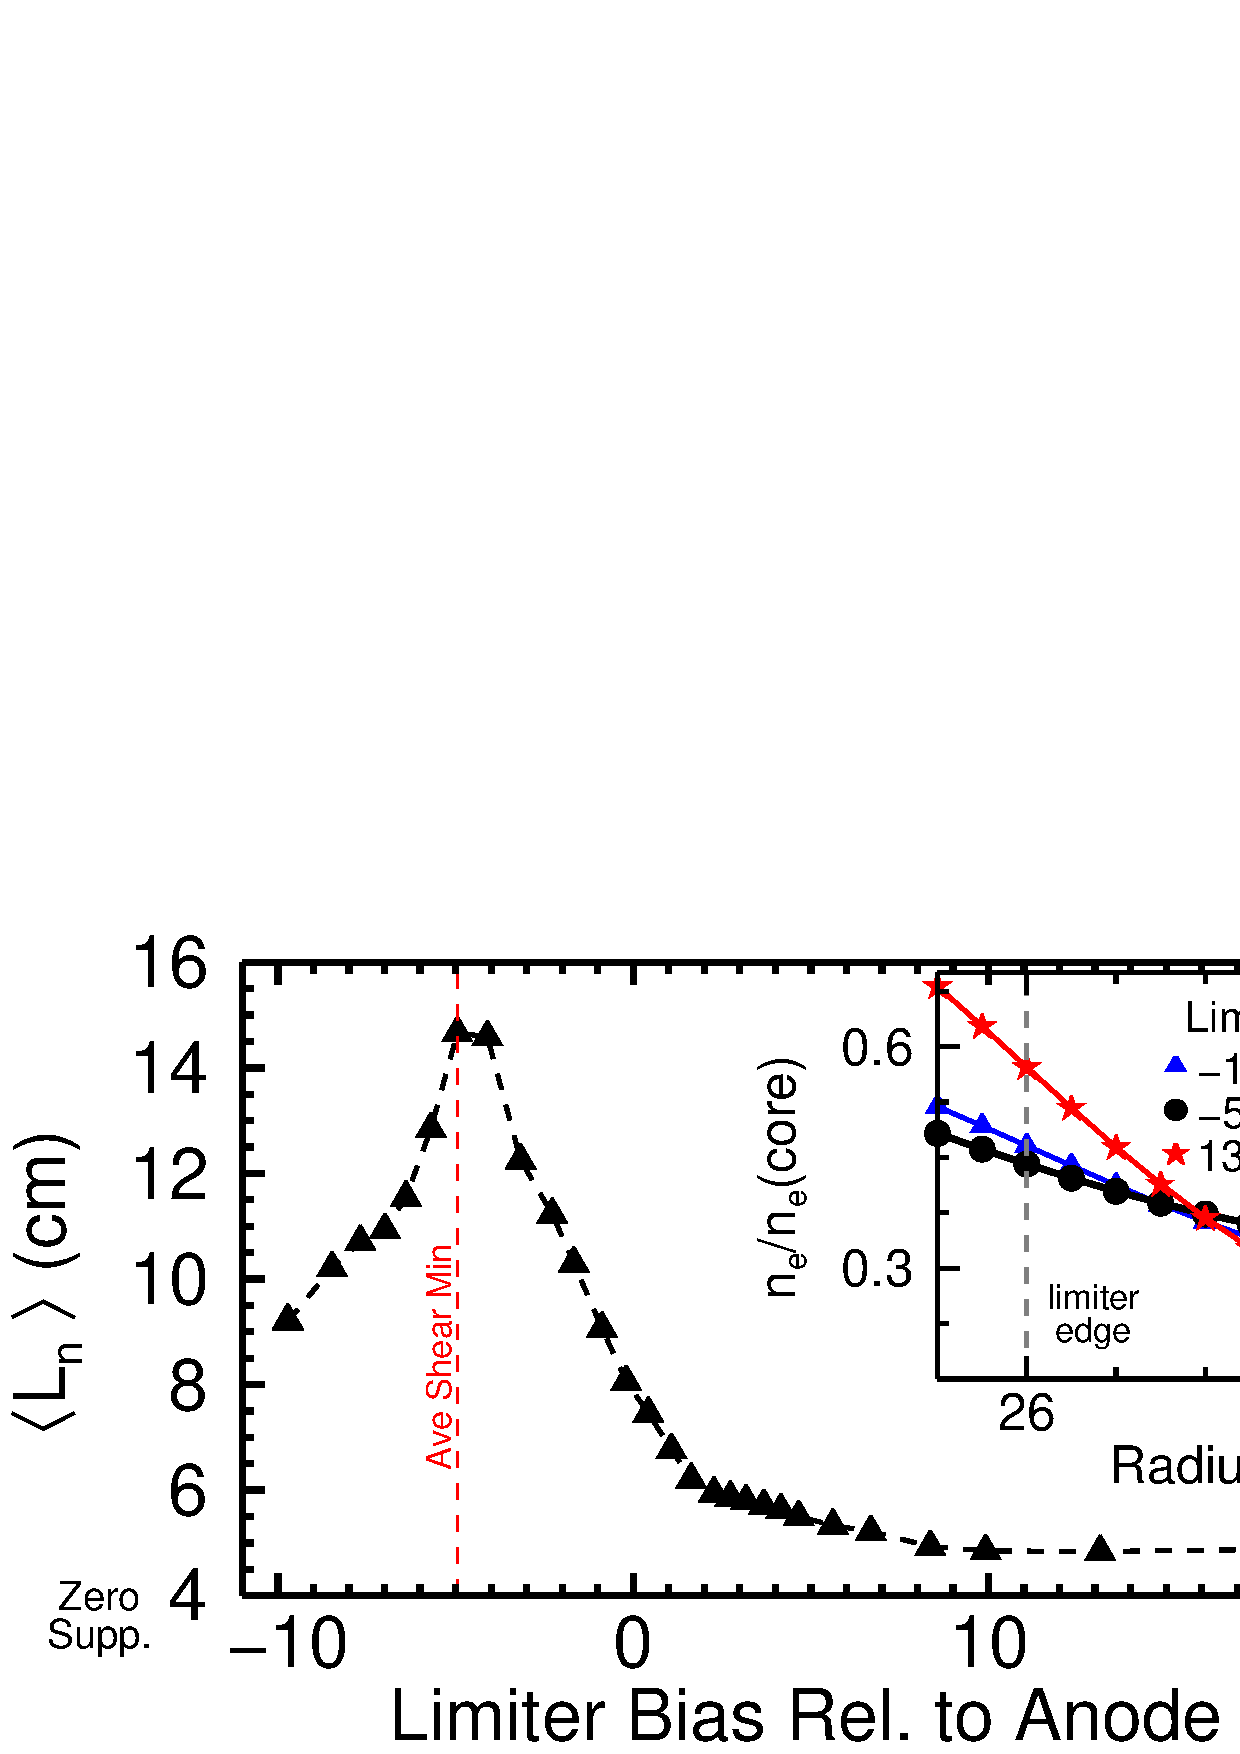
\includegraphics[width=8.5cm]{densgrad.pdf}}
\caption{\label{fig:densgrad} Density gradient length scale versus limiter bias. Inset shows density profile relaxing then steepening again with bias.}
\end{figure}

Fig.~\ref{fig:densgrad} shows the variation in the spatially-averaged density gradient length scale, $L_{n} = \lvert \nabla \ln n \rvert ^{-1}$ with
increasing limiter bias.  As the limiter bias is increase, reducing
the IDD flow, an increase in the gradient scale length is observed,
indicating a degradation of radial particle confinement which peaks
when the averaged shearing rate is near zero.  
%The first clear result is a degredation of confinement from the
%spontaneous state followed by improved confinement as bias is
%increased, as indicated by $\langle L_{n}\rangle$ in
%Fig.~\ref{fig:densgrad}. Beginning at 9cm with no bias, $\langle
%L_{n}\rangle$ reaching a scale length peak of about 15cm at the bias
%corresponding to zero shear. 
As the bias is
increased further, reversing the flow and again increasing the
shearing rate, the density gradient gradually steepens and the
scale length is lowered, indicating improved particle confinement.  

\begin{figure}[!htbp]
\centerline{
\includegraphics[width=8.5cm]{shearandgrad.pdf}}
\caption{\label{fig:shearandgrad} Gradient scale length versus shearing rate. Inset shows correlation of gradient scale length and turbulent particle flux. Note how this data is inconsistant with a Fick's Law like diffusion, which would be identified by a linearly increasing flux with gradient.}
\end{figure}


%, eventually saturating to a . The initial scale length value and saturated values are consistent with previous biasing experiments done on the LAPD\cite{carter09}, but rather than see a gradual change like here, a sharp threshold was observed. This gradual transition can be observed beause the new design allows for continous variation of flow at the plasma edge. In the previous experiment, a threshold was observed not because of an inherent dependence on a shear value, but because of lack of penetration of cross-field current---and thus flow---from the chamber edge to the plasma source until a high enough bias was reached. By placing the limiters closer to the core plasma edge edge, we can establish cross-field currents at lower bias values than before.

The observed variation of $\langle L_{n} \rangle$ with bias is best organized when compared to the average shearing rate, $\omega_s$ as is shown in Fig.~\ref{fig:shearandgrad}.   The shearing rate is normalized to the autocorrelation rate of $I_{\rm sat}$ fluctuations measured in the zero-shear state.  An autocorrelation rate of $\Delta \omega_{d} \approx $ 28kHz is calculated by taking the half-width at half-maximum of a Hilbert transform of the $I_{\rm sat}$ autocorrelation function.  Confinement improvement (decreased $\langle L_n \rangle$) occurs continuously and gradually with increasing $\omega_{s}$ and reaches saturation for $\omega_{s} \approx \Delta \omega_{d}$ (normalized $\omega_s$ of 1).  The confinement improvement appears to be largely independent of flow (or radial electric field) direction as IDD (filled points) and EDD (open points) flow cases follow the same trend when plotted against normalized shearing rate.




The change in confinement can be connected to a change in the fluctuation characteristics which dictate the turbulent flux. Fluctuation power in $I_{\rm sat}$ can be seen in the spectrum of Fig.~\ref{fig:powercontour}
\begin{figure}[!htbp]
\centerline{
\includegraphics[width=8.5cm]{powercontour.pdf}}
\caption{\label{fig:powercontour} Contour plot of log $I_{\rm sat}$ fluctuation power versus shearing rate and frequency. Dashed lines show location of decorrelation rate.}
\end{figure}
Most of the power is located in frequencies $<10$kHz and in this range, power decreases overall with increasing shearing rate. A decrease of about one order of magnitude is seen between the lowest shearing point and the high shear regime. Above 10kHz, power drops off considerably; however, just beyond $\omega_{s} = \Delta \omega_{s}$, a coherent mode emerges with a frequency that begins at about 10kHz and increases linearly with shearing. The power at these high shearing rates is almost entirely located within this mode.


 from $I_{\rm sat}$ radial profiles while particle flux, $\Gamma_{p} = \langle \tilde{n} \tilde{v_{r}} \rangle = \langle \tilde{n} \tilde{E_{\theta}} \rangle /B$, can be calculated spectrally as\cite{powers74}, 
\begin{equation}
\Gamma_{p} = \frac{2}{B} \int^{\infty}_{0} \lvert n(\omega) \rvert \lvert E_{\theta}(\omega) \rvert \gamma_{n,E_{\theta}}(\omega) \cos [\phi_{n,E_{\theta}}(\omega)] d\omega
\label{eq:fluxint}
\end{equation}
which allows for separate analysis of fluctuations, crossphase and coherency.




The changes in $L_{n}$ and fluctuations are indicative of an overall change in particle flux. This flux can be directly measured by correlating $I_{\rm sat}$ with radial flow---$E \times B$ flow---using an $E_{\theta}$ derived from two floating potential tips on either side of the $I_{\rm sat}$ measuring tip and rewritten in terms of the integral in \eqref{eq:fluxint}. Like $L_{n}$, flux decreases with shearing rate as in Fig.~\ref{fig:fluxvsshear}; however, while flux decrease begin immediately with shearing, the decrease is not as fast as $L_{n}$ with saturation not occuring until at least $\omega_{s} > 2\Delta \omega_{d}$. Flux decreases do not depend on flow direction either as again both IDD and EDD points fit on the same curve.

\begin{figure}
\begin{center}
\includegraphics[width=8.5cm]{fluxvsshear.pdf}% Here is how to import EPS art
\caption{\label{fig:fluxvsshear} Particle flux normalized to no-shear flux as a function of normalized shearing rate. Filled symbols represent points with flow in IDD.}
\end{center}
\end{figure}

%When the flux is bandwidth limited, a difference emerges. The flux from 350Hz to 10kHz, where most of the fluctuation power is located, drops off gradually, %hitting its minimum only at a shearing rate about three times the decorrelation rate. Higher bandwidth though, 10kHz to 50kHz, drops off faster, nearing its %minimum when shearing equals decorrelation rate. Best fit lines from log-log plots of these scatters using a power law form of $\left(\omega_{s}/\Delta %\omega_{t}\right)^{\alpha}$ yield exponents of $\alpha = -0.887$ for the low bandwidth flux and about $\alpha = -1.008$ for the high bandwidth flux. 

\begin{figure}
\begin{center}
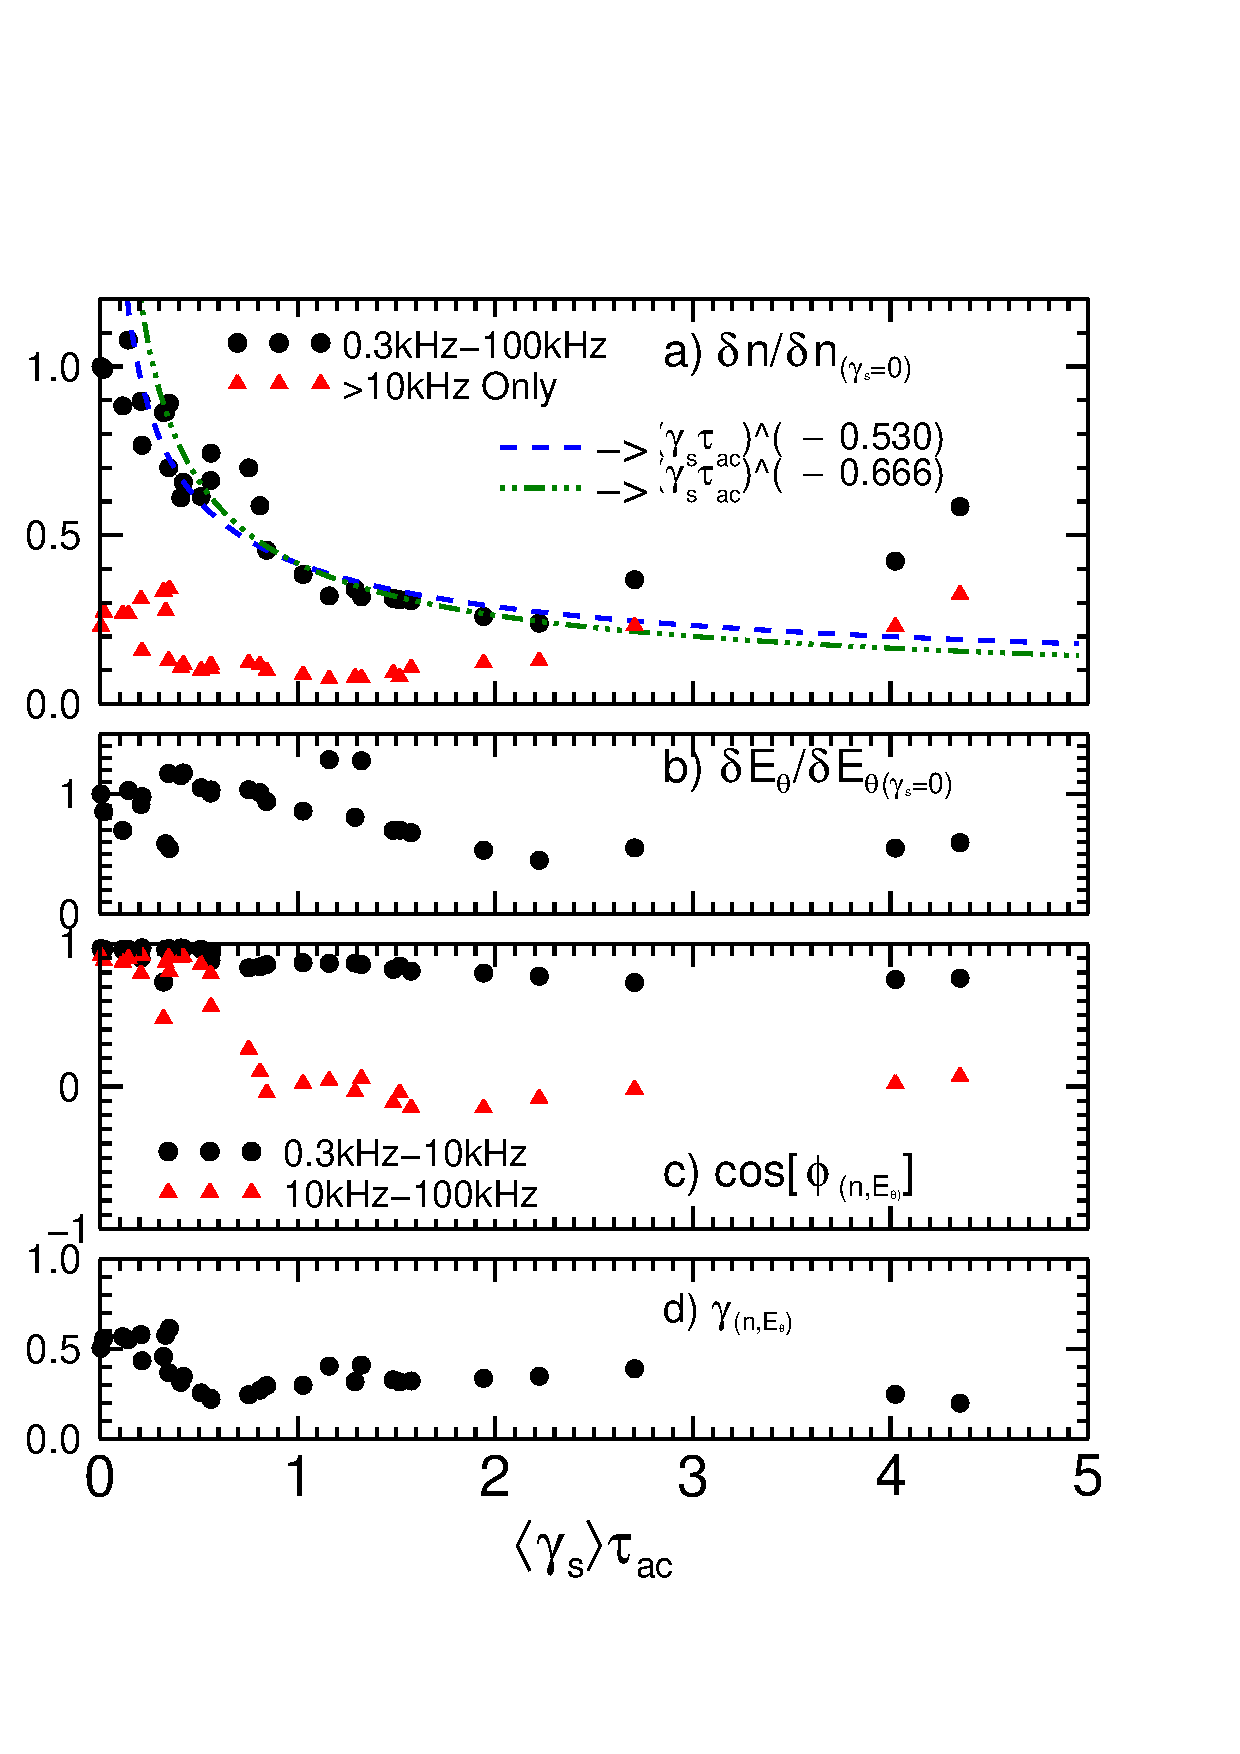
\includegraphics[width=8.5cm]{fluxcomps.pdf}% Here is how to import EPS art
\caption{\label{fig:fluxcomps} Components of particle flux versus shearing rate including $I_{\rm sat}$/Density fluctuation power(a), electric field fluctuation power(b), crossphase(c) and coherency(d) with black points for low frequency, red for high.}
\end{center}
\end{figure}

\begin{figure}
\begin{center}
\includegraphics[width=8.5cm]{radcorr.pdf}% Here is how to import EPS art
\caption{\label{fig:radcorr} Radially correlation lengths with reference probes at 28,29,30,31 or 32cm. Inset shows 2D correlation structure for IDD flow, no shear and high EDD flow. A mode pattern is seen at flow peak (26cm).}
\end{center}
\end{figure}

The calculated flux can be analyzed by its fluctuation and phase components separately as in Fig.~\ref{fig:fluxcomps}. The top two plots show fluctuation power---$I_{\rm sat}$ and azimuthal electric field ($E_{\theta}$)---as functions of normalized shearing rate, while the bottom two show crossphase and coherency between the two fluctuating quantities. As expected from the power contour plot, $I_{\rm sat}$ fluctuations decrease with shearing for frequencies $<10$kHz. Concurrently, $\cos(\phi_{I_{\rm sat},E_{\theta}})$ for this bandwidth remains steady at nearly 1.0. Thus, since fluctaution power is concentrated in the low frequencies, overall flux is predominately suppressed by decreases in $I_{\rm sat}$ fluctuations, not crossphase. Note, however, $I_{\rm sat}$ fluctuations appear to increase beyond a normalized shearing of 2.0. These increases, however, are almost entirely from $>10$kHz contributions suggesting that they originate from the coherent mode. Comparing to Fig.~\ref{fig:fluxvsshear}, it is clear these flucutations do not contribute significantly to the flux. For high frequencies $\cos(\phi_{I_{\rm sat},E_{\theta}})$ is nearly zero for $\omega_{s} > \Delta \omega_{d}$. Thus, despite increased fluctuations at high shear, no overall flux is observed. 

%For low bandwidth, $I_{\rm sat}$ power decreases gradually, with a power fit of $\alpha = 0.581$. Crossphase, on the other hand, does not decrease. In this bandwidth %then, decreases in flux are primarily due to decreasing turbulent power. For high bandwidth flux, though, the opposite appears to be true. While $I_{\rm sat}$ %fluctuations do decrease initially, they actually begin to increase at high shearing rates. In this case, flux suppression is primarily due to the drop in %crossphase and to some extent coherency, regardless of growing turbulent power. A fit to this high frequency crossphase calculation yields $\alpha = -3.021$.  %Electric field fluctuations, meanwhile, appear to be mostly unaffected by shearing. For both high and low frequency, the fluctuation power is reduced by no more %than 50\% with even the highest shearing achieved. For comparison to BDT theory, a curve of power $\alpha = -(2/3)$ is plotted for $I_{\rm sat}$ fluctuations, while a %curve of power $\alpha = -(8/3)$, two powers larger than $-(2/3)$, is show for the crossphase plot.


As predicted by early theories on shear suppression, the effect of decreasing fluctuations is related to the shortening of a radial correlation length, $\Delta r_{c}$, for turbulent structures. Using a cross-correlation technique, we observe this modification of structures by azimuthal shearing as shown in Fig.~\ref{fig:radcorr}. $\Delta r_{c}$ is defined as the width of the contour plot at one-half its value at the reference point, represented by the black curve in the inset of Fig.~\ref{fig:radcorr}. Like the flux and fluctuation data, the suppression begins with relatively little shearing and approaches a saturated value, though unlike flux, there appears to be a slight asymmetry in widths for IDD and EDD. This may be due to the influence of the coherent mode. In the high shearing regime shown in inset c) of Fig.~\ref{fig:radcorr}, a mode pattern is observed in the peak EDD flow region and is distinct from the correlation structure. A similar, more diffuse mode may be present in the IDD flow region, but is more difficult to distinguish from the correlation structure thus adding to the apparent $\Delta r_{c}$.

Lastly, we can compare some of our results to theory. Considering the effect of shearing on eddy step size, the BDT model \cite{biglari90} predicts a power-law scaling of the form $\left(\omega_{s}/\Delta \omega_{t}\right)^{-\alpha}$ for $\tilde{n}$ and $\Delta r_{c}$. A comparison of the power fit to the predicted exponent is made for each quantity. As seen in Fig.~\ref{fig:fluxcomps} a best fit of $\alpha = 0.530$ compares favorably to the BDT prediction of $\alpha = 2/3$. Similarly, a fit of $\alpha = 0.461$ for $\Delta r_{c}$ in Fig.~\ref{fig:radcorr} compares well to the BDT prediction of $\alpha = 1/3$. A cavaet: BDT theory is based on a constant density gradient while here gradients are always changing. Nevertheless, this initial agreement of data to model is promising for future comparisons.

%The correlation lengths can also be separated by frequency. Note how IDD flow structures appear to grow someone wider with shear rather than EDD flow structures %as show by the filled symbols. This may be due to contributions from a growing coherent mode with shear which is much more apparent and distinct in the EDD flow %direction. 

%This correlation length decreases with shearing rate roughly following a power-law with $\alpha = -(1/3)$ indicating the sheared flow's ability to decrease the %radial extend of a turbulent eddy.

This letter presents the first continous variation shearing rate in a plasma device and has shown a clear effect of particle flux and density confinement through both the mechanisms of turbulent fluctuation and radial correlation length reduction.

%\nocite{*}
\bibliography{FlowModPRL_bib}% Produces the bibliography via BibTeX.

\end{document}
%
% ****** End of file aipsamp.tex ******
